\documentclass[preprint,12pt,aps,pra,showkeys,amsmath,amssymb,superscriptaddress,floatfix]{revtex4-2}
\usepackage[T1]{fontenc}
\usepackage[utf8]{inputenc}
\usepackage{amsmath,amssymb,amsthm,mathtools,mathrsfs}
\usepackage{microtype,booktabs,enumitem}
\usepackage{xcolor,tikz,etoolbox}
\usepackage[skins,breakable]{tcolorbox}
\usepackage{needspace}
% Keep diagram geometry independent of REVTeX preprint body spacing.
\AtBeginEnvironment{tikzpicture}{\linespread{1}\selectfont}
\usetikzlibrary{arrows.meta,positioning,calc,fit,decorations.pathreplacing}
\usepackage{graphicx}
\usepackage{hyperref}

\definecolor{MMBlue}{RGB}{0,82,155}
\definecolor{MMOrange}{RGB}{200,80,0}
\tikzset{
 mmnode/.style={draw=MMBlue,rounded corners=2pt,fill=MMBlue!4,align=left,execute at begin node={\raggedright},text width=5cm,font=\fontsize{10}{12}\selectfont,inner sep=6pt},
 mmimport/.style={mmnode,draw=black!65,fill=black!4},
 mmcandidate/.style={mmnode,draw=MMOrange,dashed,fill=MMOrange!5},
 mmrejected/.style={mmnode,draw=black,densely dotted,fill=black!8},
 mmproof/.style={->,thick,MMBlue},
 mmflow/.style={->,semithick,black!70},
 mmrepair/.style={->,dashed,thick,MMOrange},
 mmcandidatearrow/.style={->,dashed,semithick,MMOrange},
 mmnote/.style={font=\scriptsize,fill=white,inner sep=2pt,align=center}}

\usepackage[section]{placeins}
\setlength{\emergencystretch}{3em}
\setlist{itemsep=3pt,topsep=4pt}
\newtheorem{theorem}{Theorem}[section]
\newtheorem{proposition}[theorem]{Proposition}
\newtheorem{lemma}[theorem]{Lemma}
\newtheorem{corollary}[theorem]{Corollary}
\theoremstyle{definition}
\newtheorem{definition}[theorem]{Definition}
\newtheorem{example}[theorem]{Example}
\theoremstyle{remark}
\newtheorem{remark}[theorem]{Remark}
% Avoid isolated statement headings and single-line paragraph fragments.
\BeforeBeginEnvironment{theorem}{\Needspace{6\baselineskip}}
\BeforeBeginEnvironment{definition}{\Needspace{5\baselineskip}}
\BeforeBeginEnvironment{proposition}{\Needspace{5\baselineskip}}
\BeforeBeginEnvironment{lemma}{\Needspace{5\baselineskip}}
\BeforeBeginEnvironment{corollary}{\Needspace{5\baselineskip}}
\clubpenalty=5000
\widowpenalty=5000
\newcommand{\R}{\mathbb R}\newcommand{\Z}{\mathbb Z}\newcommand{\N}{\mathbb N}
\newcommand{\Pa}{\operatorname{Pa}}\newcommand{\Desc}{\operatorname{Desc}}
\newcommand{\cl}{\operatorname{cl}}\newcommand{\cost}{\operatorname{cost}}
\newcommand{\status}{\operatorname{status}}
% Faculty cards: a visual rail groups the five faculties within one agent.
% The rail has no arrowhead and does not represent a proof dependency.
\newcommand{\mmfacultybadge}[1]{%
 \node[circle,draw=MMBlue,line width=1pt,fill=white,
 minimum size=7mm,inner sep=0pt,font=\sffamily\small\bfseries,text=MMBlue]
 at ([xshift=15pt,yshift=-15pt]frame.north west) {#1};}
\newcommand{\mmfacultyrail}{%
 \draw[MMBlue!80,line width=1pt]
 ([xshift=15pt,yshift=2pt]frame.north west)--
 ([xshift=15pt,yshift=-2pt]frame.south west);}
\newtcolorbox{mmfacultybox}[2]{enhanced,breakable,
 colback=MMBlue!4,colframe=MMBlue!4,boxrule=0pt,arc=3pt,
 left=39pt,right=9pt,top=4pt,bottom=4pt,
 before skip=2pt,after skip=2pt,
 fontupper=\small\linespread{1.1}\selectfont,
 overlay unbroken={\mmfacultyrail\mmfacultybadge{#1}},
 overlay first={\mmfacultyrail\mmfacultybadge{#1}},
 overlay middle={\mmfacultyrail},overlay last={\mmfacultyrail}}
\newcommand{\mmfaculty}[3]{%
 \begin{mmfacultybox}{#1}{#2}
 {\sffamily\bfseries\color{MMBlue}#2}\par\smallskip #3
 \end{mmfacultybox}}
\newcommand{\agent}[9]{%
 \Needspace{8\baselineskip}
 \subsubsection{#1}
 \noindent\textbf{Object.} #2\par
 \noindent\textbf{Role.} #3\par\smallskip
 \mmfaculty{E}{Ego}{#4}
 \mmfaculty{M}{Memory}{#5}
 \mmfaculty{I}{Intellect}{#6}
 \mmfaculty{S}{Sense}{#7}
 \mmfaculty{A}{Action}{#8}
 \smallskip\noindent #9\par}

\usepackage{longtable,array,calc}
\providecommand{\tightlist}{\setlength{\itemsep}{2pt}\setlength{\parskip}{0pt}}
\makeatletter
\def\frontmatter@abstract@produce{\par\addvspace{\frontmatter@preabstractspace}%
\begingroup\prep@absbox\unvbox\absbox\post@absbox\endgroup
\addvspace{\frontmatter@postabstractspace}}
\makeatother
\newcommand{\field}[2]{\par\smallskip\noindent\textbf{#1.} #2\par}
\setlength{\emergencystretch}{5em}
\AtBeginEnvironment{verbatim}{\small\linespread{1.0}\selectfont}


\hypersetup{colorlinks=true,linkcolor=MMBlue,urlcolor=MMBlue,pdfauthor={Dibakar Sigdel}}

\begin{document}

\title{Composite Trapezoidal Rule with a Certified Error Bound\\[4pt]\large An End-to-End Meta-Math Walkthrough}

\author{Dibakar Sigdel}

\affiliation{Mindverse Computing LLC, Lynnwood, WA 98087, USA}

\date{October 2026}

\begin{abstract}

A nonnegative kernel expresses the local quadrature error exactly. Its
integral gives the constant, and summing local errors gives the global
order. The report presents the target theorem, declared imports, a
dependency graph, five-faculty node contracts, a continuous proof, a
worked example, and a hypothesis-repair audit. It is an authored
mathematical exposition, not a deployed-agent transcript or a formal
proof-assistant certificate.

\end{abstract}\maketitle\linespread{1.12}\selectfont

\noindent\textbf{ON-05 / Optimization and Numerical Analysis / Report v1}

\section{Target and import contract}

\begin{theorem}

For \(f\in C^2([a,b])\), \(a<b\), let \(N\ge1\), \(h=(b-a)/N\), and
\(x_j=a+jh\). Define \(T_N=h(f(a)/2+\sum_{j=1}^{N-1}f(x_j)+f(b)/2)\).
Prove \(|T_N-\int_a^b f(x)\,dx|\le (b-a)h^2\|f''\|_\infty/12\). If
\(f''\ge0\), also prove \(T_N\ge\int_a^b f\). These concern exact
sampled values and arithmetic.

\end{theorem}

\subsection{Foundations and permitted imports}

Use integration by parts for \(C^2\) functions and finite sums. The
bound \(\|f''\|_\infty\) is finite by continuity on the compact
interval. Distinguish quadrature error from errors in function
evaluation or floating-point summation, which require separate
estimates.

\clearpage\section{Node interaction workflow}

\begin{center}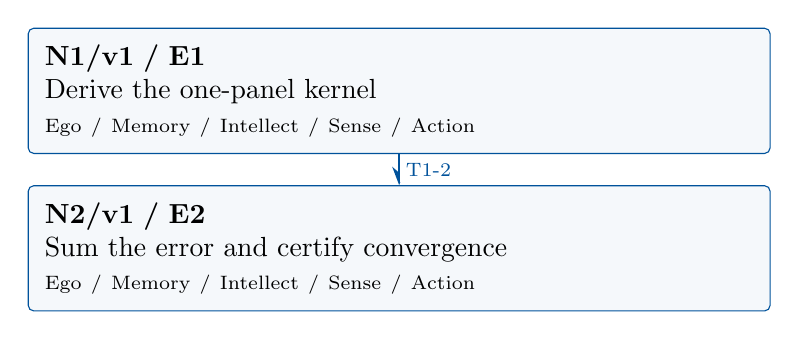
\begin{tikzpicture}[>=Stealth,x=1cm,y=1cm]

\node[mmnode,text width=9cm,minimum height=1.25cm] (N1) at (0,0.0) {\textbf{N1/v1 / E1}\\Derive the one-panel kernel\\{\scriptsize Ego / Memory / Intellect / Sense / Action}};

\node[mmnode,text width=9cm,minimum height=1.25cm] (N2) at (0,-2.0) {\textbf{N2/v1 / E2}\\Sum the error and certify convergence\\{\scriptsize Ego / Memory / Intellect / Sense / Action}};

\draw[mmproof] (N1.south) -- node[mmnote,right] {T1-2} (N2.north);

\end{tikzpicture}\end{center}

Each box is one mathematical agent containing all five faculties. Blue
arrows carry the versioned exports listed below. The layout gives a
reading order; only drawn arrows assert dependencies. Diagnostic repair
is separate from the proof DAG.

\subsection{Versioned evidence-transfer ledger}

\begingroup\small\linespread{1.05}\selectfont

\Needspace{5\baselineskip}\field{T1-2: N1/E1/v1 to N2}{\(\frac h2(f(u)+f(v))-\int_u^v f=\int_u^v K(t)f''(t)\,dt\).}

\field{Receiving activity}{N2.1}

\field{Compatibility}{E1/v1 on each of the \(N\) equal panels. Check: There are \(N=(b-a)/h\)
panels, so the local \(h^3\) bound becomes a global \(h^2\) bound.}

\endgroup

\clearpage\section{Agent roles and five-faculty activities}\begingroup\small\linespread{1.05}\selectfont\setlist{itemsep=1pt,topsep=2pt}

\subsection{N1/v1: Derive the one-panel kernel}

\field{Object and role}{Integrate \(Kf''\) twice by parts to recover endpoint weights and the
exact integral. \textbf{Local obligation:}
\(\frac h2(f(u)+f(v))-\int_u^v f=\int_u^v K(t)f''(t)\,dt\).}

\field{Inputs}{One interval \([u,v]\) of length \(h\) and \(K(t)=(t-u)(v-t)/2\).}

\mmfaculty{E}{Ego}{Publish E1/v1 only after establishing this obligation:
\(\frac h2(f(u)+f(v))-\int_u^v f=\int_u^v K(t)f''(t)\,dt\).}

\mmfaculty{M}{Memory}{One interval \([u,v]\) of length \(h\) and \(K(t)=(t-u)(v-t)/2\). Retain
the stated assumptions and import versions.}

\mmfaculty{I}{Intellect}{Integrate \(Kf''\) twice by parts to recover endpoint weights and the
exact integral.}

\mmfaculty{S}{Sense}{The boundary values are \(K(u)=K(v)=0\), \(K'(u)=h/2\), \(K'(v)=-h/2\),
and \(K''=-1\).}

\mmfaculty{A}{Action}{Carry out activities N1.1--N1.2 below, retaining each calculation and
construction as evidence.}

\smallskip\noindent\textbf{Numbered mathematical activities}

\begin{enumerate}[label=N1.\arabic*,leftmargin=3.4em]

\item Integration by parts gives \(\int_u^v Kf''=-\int_u^v K'f'\), since \(K\)
vanishes at the endpoints. Integrating again gives
\(-[K'f]_u^v+\int_u^v K''f\).

\item Using the displayed endpoint derivatives and \(K''=-1\) yields
\((h/2)(f(u)+f(v))-\int_u^v f\), exactly the local error with the sign
\(T-I\). Also \(K\ge0\) and, after setting \(s=t-u\),
\(\int_u^v K=\frac12\int_0^h s(h-s)\,ds=h^3/12\).

\end{enumerate}

\field{Export E1/v1}{\(\frac h2(f(u)+f(v))-\int_u^v f=\int_u^v K(t)f''(t)\,dt\).}

\field{Acceptance gate}{The boundary values are \(K(u)=K(v)=0\), \(K'(u)=h/2\), \(K'(v)=-h/2\),
and \(K''=-1\).}

\field{Targeted repair}{If the sign of the error is uncertain, recompute the endpoint
derivatives of \(K\) before taking absolute values. Withhold this export
and recheck its descendants after a versioned correction.}

\clearpage

\subsection{N2/v1: Sum the error and certify convergence}

\field{Object and role}{Add exact identities, then use nonnegativity of the kernel for magnitude
and sign. \textbf{Local obligation:} The stated absolute error and
convex-function overestimate hold; in particular \(T_N\to\int_a^b f\).}

\field{Inputs}{E1/v1 on each of the \(N\) equal panels. Incoming proof exports: E1/v1
at N2.1.}

\mmfaculty{E}{Ego}{Publish E2/v1 only after establishing this obligation: The stated
absolute error and convex-function overestimate hold; in particular
\(T_N\to\int_a^b f\).}

\mmfaculty{M}{Memory}{E1/v1 on each of the \(N\) equal panels. Incoming proof exports: E1/v1
at N2.1. Retain the stated assumptions and import versions.}

\mmfaculty{I}{Intellect}{Add exact identities, then use nonnegativity of the kernel for magnitude
and sign.}

\mmfaculty{S}{Sense}{There are \(N=(b-a)/h\) panels, so the local \(h^3\) bound becomes a
global \(h^2\) bound.}

\mmfaculty{A}{Action}{Carry out activities N2.1--N2.2 below, retaining each calculation and
construction as evidence.}

\smallskip\noindent\textbf{Numbered mathematical activities}

\begin{enumerate}[label=N2.\arabic*,leftmargin=3.4em]

\item Summing the one-panel trapezoids counts each interior sample twice with
weight \(h/2\), producing \(T_N\). The exact error is the sum of the
panel kernel integrals. Its absolute value is bounded by
\(N(h^3/12)\|f''\|_\infty=(b-a)h^2\|f''\|_\infty/12\).

\item If \(f''\ge0\), every kernel integral is nonnegative, proving the
overestimate. Since \(h\to0\) as \(N\to\infty\), the absolute bound also
proves convergence. The smoothness and fixed interval make the same
derivative bound valid for all \(N\).

\end{enumerate}

\field{Export E2/v1}{The stated absolute error and convex-function overestimate hold; in
particular \(T_N\to\int_a^b f\).}

\field{Acceptance gate}{There are \(N=(b-a)/h\) panels, so the local \(h^3\) bound becomes a
global \(h^2\) bound.}

\field{Targeted repair}{If the local \(h^3\) rate is reported as the global rate, multiply by
the number of panels and restore the \(h^2\) bound. Withhold this export
and recheck its descendants after a versioned correction.}

\endgroup\clearpage\section{Continuous mathematical proof}\label{sec:proof}

\subsection{N1 --- Derive the one-panel
kernel}\label{n1-derive-the-one-panel-kernel}

\begin{enumerate}
\def\labelenumi{\arabic{enumi}.}
\item
  \textbf{N1.1.} Integration by parts gives
  \(\int_u^v Kf''=-\int_u^v K'f'\), since \(K\) vanishes at the
  endpoints. Integrating again gives \(-[K'f]_u^v+\int_u^v K''f\).
\item
  \textbf{N1.2.} Using the displayed endpoint derivatives and \(K''=-1\)
  yields \((h/2)(f(u)+f(v))-\int_u^v f\), exactly the local error with
  the sign \(T-I\). Also \(K\ge0\) and, after setting \(s=t-u\),
  \(\int_u^v K=\frac12\int_0^h s(h-s)\,ds=h^3/12\).
\end{enumerate}

\subsection{N2 --- Sum the error and certify
convergence}\label{n2-sum-the-error-and-certify-convergence}

\begin{enumerate}
\def\labelenumi{\arabic{enumi}.}
\item
  \textbf{N2.1.} Summing the one-panel trapezoids counts each interior
  sample twice with weight \(h/2\), producing \(T_N\). The exact error
  is the sum of the panel kernel integrals. Its absolute value is
  bounded by \(N(h^3/12)\|f''\|_\infty=(b-a)h^2\|f''\|_\infty/12\).
\item
  \textbf{N2.2.} If \(f''\ge0\), every kernel integral is nonnegative,
  proving the overestimate. Since \(h\to0\) as \(N\to\infty\), the
  absolute bound also proves convergence. The smoothness and fixed
  interval make the same derivative bound valid for all \(N\).
\end{enumerate}

\hfill$\square$

\section{Worked orchestration}

For \(f(x)=x^2\) on \([0,1]\) and \(N=2\),
\(T_2=\tfrac12(0+\tfrac14+\tfrac12)=3/8\), while the integral is
\(1/3\). The error is \(1/24\), exactly the bound
\(1\cdot(1/2)^2\cdot2/12=1/24\). Convexity correctly predicts an
overestimate.

\subsection{Boundary and hypothesis audit}

For \(f(x)=|x|\) on \([-1,1]\), the one-panel trapezoid is \(2\) and the
integral is \(1\). Although \(f''=0\) away from zero, the function is
not \(C^2\); treating its a.e. second derivative as a classical uniform
bound would incorrectly predict zero error.

\section{Illustrative failure and repair}

The following is an authored diagnostic scenario. Changed assumptions
define a new contract; they do not retroactively prove the original
statement.

\subsection{Rejected argument, diagnosis, and correction}
\textbf{Rejected N1 shortcut:} use \(f''=0\) almost everywhere in the
\(C^2\) kernel formula for \(|x|\). \textbf{Diagnosis:} Memory silently
replaced classical regularity by an a.e. derivative without the needed
absolute-continuity bridge. \textbf{Repair:} keep the stated \(C^2\)
hypothesis; for \(|x|\), split at its corner and integrate the two
affine pieces separately, obtaining the exact value \(1\). That split is
a separate valid computation, not a proof of the unqualified bound.

\subsection{Publication and reuse}
The corrected export retains its explicit assumptions. A hypothetical
revision receives a new version, and each consuming activity is
rechecked; this scenario is not a recorded runtime event. \textbf{Next
direction:} Develop adaptive panel selection from local derivative
bounds, then add explicit evaluation and roundoff error terms for
numerical certification.

\par\medskip\begingroup\small\linespread{1.0}\selectfont\noindent\textbf{Provenance.} This authored proof is complete relative to its declared imports. Reuse
each export with its assumptions, proof, and version. The original
Markdown remains available for comparison.
\par\endgroup

\par\smallskip\begingroup\small\linespread{1.0}\selectfont\noindent\textbf{Further reading.} \href{https://web.stanford.edu/~boyd/cvxbook/}{Boyd and Vandenberghe,
Convex Optimization} for convexity, optimality, and descent;
\href{https://www.math.umd.edu/~mariakc/Spring2020Class.html}{University
of Maryland, Scientific Computing I} for the numerical-analysis setting.
The estimates used here are derived explicitly in §4.\par\endgroup

\end{document}
